\documentclass[12pt]{article}

\usepackage[utf8]{inputenc}

\usepackage{graphicx}
\graphicspath{ {./images/} }
\usepackage{csquotes}
\usepackage{geometry}
\usepackage[colorlinks]{hyperref}
\hypersetup{
  linkcolor=blue,
  anchorcolor=,
  citecolor=,
  filecolor=,
  menucolor=,
  runcolor=,
  urlcolor=blue,
}
\geometry{a4paper, margin=3cm}
\font\titlefont=cmr12 at 18pt
\setlength{\parindent}{0em}

\title{\titlefont The Settlers II (10th Anniversary) - An advanced guide}
\author{TheCheese}
\date{}

\begin{document}

\maketitle

\vspace{2cm}

\begingroup
  \hypersetup{hidelinks}
  \tableofcontents
\endgroup


\section{Introduction}
\label{sec:introduction}

\begin{displayquote}
\textbf{The Settlers II (10th Anniversary)} (German: Die Siedler II: Die nächste Generation) is a city-building game with real-time strategy elements, developed by Blue Byte and published by Ubisoft. Released for Microsoft Windows in September 2006, it is a remake of The Settlers II (1996).
\end{displayquote}
\hspace{2cm}- \textit{\href{https://en.wikipedia.org/wiki/The_Settlers_II_(10th_Anniversary)}{Wikipedia}}\\

This guide is not just about getting started with the game, as well as some tricks and tips, but also aims to cover more advanced techniques and strategies, along with specialized optimizations and common pitfalls. The main part is focussed only on the base version of the game. However, there is a \hyperref[sec:vikings]{bonus category} on the Vikings addon. Have fun reading!

\subsection{Contributing}
\label{sec:contributing}

This guide's \LaTeX-code is available on GitHub. If you want to add something, found out something new or just want to report false content, please submit a pull request or open an issue: \url{https://github.com/TheCheese42/ts2-anniversary-guide}.

\section{Installation}
\label{sec:installation}

The game can be bought from the GOG.com store \href{https://www.gog.com/en/game/the_settlers_2_10th_anniversary}{here}. Despite only supporting Microsoft Windows, playing it on UNIX systems like MacOS or Linux is no problem thanks to compatibility layers like \href{https://www.winehq.org}{Wine}.

\section{Getting Started}
\label{sec:gettingstarted}

The following covers common actions needed to get a good start into a new game.

\subsection{Road System}
\label{sec:roadsystem}

The most straightforward way to connect buildings is simply putting roads everywhere so everything is connected somehow. While this can work on small maps or poor economies, it's way more efficient to use a grid system. See the image below.

\vspace{12pt}
\includegraphics[width=\textwidth]{perfect_roadsystem_crop}
\vspace{0pt}

As you can see, there is no problem including any buildings (except for \hyperref[sec:harbor]{harbors}) into this road grid. It even perfectly fits the \hyperref[sec:farm]{Farm}, as it enforces its optimal layout. Usually, it's a good idea to always stick with this system, even when taking up enemy buildings. Those may take 2 or even 4 building spots instead of one as they probably aren't in your grid pattern, however, including them anyway will most certainly pay off when raising an independent industry in the newly gained territory. Below is another example showing a fully working independent food- and wood industry using this grid.

\vspace{12pt}
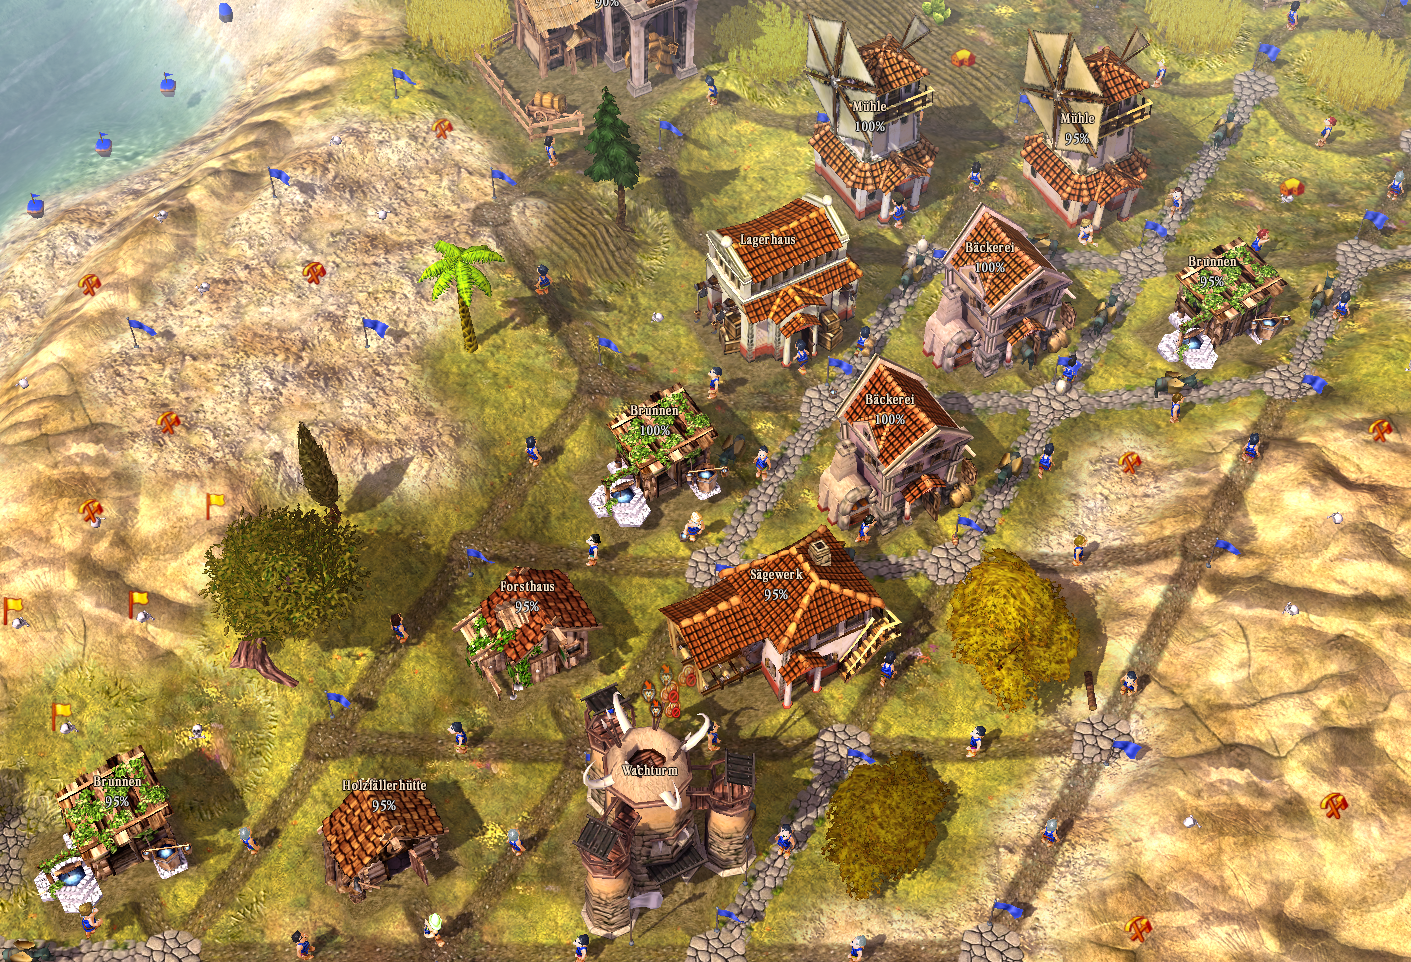
\includegraphics[width=\textwidth]{roadsystem_in_use_crop}

\subsection{Wood industry}
\label{sec:woodindustry}

The first thing you'll need is enough wood to expand using barracks and to build Mines, together with a solid food industry.

The \hyperref[sec:woodcutter]{Woodcutter} and the \hyperref[sec:forester]{Forester} both produce about 60 items per hour, while the \hyperref[sec:sawmill]{Sawmill} produces 80 items per hour. Therefore, it's best to use 4 \hyperref[sec:woodcutter]{Woodcutters} and \hyperref[sec:forester]{Foresters} with 3 \hyperref[sec:sawmill]{Sawmills}. If you need more, add 1 to every of those, however, this setup is very sufficient most of the time, unless you need to make a big fleet of \hyperref[sec:ships]{Ships} right at the beginning.

\subsection{Expanding}
\label{sec:expanding}

To have more space for your industry and to reach more mining spots, as well as pushing the enemy, you will need to expand your territory as quickly as possible. \hyperref[sec:barrack]{Barracks} are the most efficient buildings to do so, as they only require 2 planks and therefore a minimum of 60 seconds to build. You should expand in every possible direction to quickly gain a size advantage over your enemies. To speed up the process, you can use some advanced mechanics, like using \hyperref[sec:ghostbuildings]{ghost buildings}.

\subsection{Mines and Food}
\label{sec:minesandfoot}

The first mining resource you'll need is gold. If you are the first one to find and use gold, you can quickly overcome the nearest enemy. To upgrade your soldiers, you need a \hyperref[sec:mint]{Mint}, that requires one gold and one coal per coin. The production speed of a \hyperref[sec:mine]{Mine} and a \hyperref[sec:mint]{Mint} is in both cases 49 seconds per item, so you need exactly one \hyperref[sec:coalmine]{Coal-} and one \hyperref[sec:goldmine]{Gold Mine} to keep a \hyperref[sec:mint]{Mint} running. Most of the time, 2 \hyperref[sec:mint]{Mints} are enough for a run, so you'll want to not have more than 2 \hyperref[sec:goldmine]{Gold Mines} running at a time. Make sure you spread those as much as possible to avoid having to destroy them again early.

Depending on your \hyperref[sec:startresources]{starting resources}, you might need to make new tools. As you already have between 8 and 32 iron in your headquarter, you should use that for your \hyperref[sec:toolmaker]{Toolmaker} and turn his production off after the materials are used up, assuming you don't need any further tools.

The next type of \hyperref[sec:mine]{Mine} you will need is an \hyperref[sec:ironmine]{Iron Mine} to make new soldiers. A \hyperref[sec:smithy]{Smithy} requires one iron and one Coal per weapon. To get iron, you also demand a \hyperref[sec:smeltery]{Smeltery}, which requires one iron ore and one coal ore per iron. As both buildings take 49 seconds to fulfill their work, you need one \hyperref[sec:ironmine]{Iron Mine} and two \hyperref[sec:coalmine]{Coal Mines} to keep a \hyperref[sec:smeltery]{Smeltery} + \hyperref[sec:smithy]{Smithy} setup running. However, it's often advisable to have \textbf{two} \hyperref[sec:smithy]{Smithies} and one \hyperref[sec:brewery]{Brewery} running, so you should double that number.

Lastly, there are \hyperref[sec:stonemine]{Stone Mines}. If you are \textbf{not} playing on low \hyperref[sec:startresources]{starting resources}, or you've got a stonecutter working, you won't need those at first. Place them as you need them.

Assuming you didn't build any \hyperref[sec:stonemine]{Stone Mines} immediately, we are at 2 \hyperref[sec:goldmine]{Gold Mines}, 2 \hyperref[sec:ironmine]{Iron Mines} and 6 \hyperref[sec:coalmine]{Coal Mines}, making 10 in total. To get all those miners working, a good \hyperref[sec:foodsystems]{food system} is essential. Also, check out this \hyperref[sec:foodsystemcomparison]{food system comparison} to decide what suits best for your particular map.

In conclusion, start by building some \hyperref[sec:fisherman]{Fisherman} and \hyperref[sec:hunter]{Hunter}, as long as it makes sense and you have enough tools.
Then continue investing in \hyperref[sec:farm]{Farms}, \hyperref[sec:mill]{Mills} and \hyperref[sec:bakery]{Bakeries} for a healthy, vegan nutrition for your fellow miners.

\subsection{Decentralization}
\label{sec:decentralization}

To avoid long transport ways you should refine your products right where they are being produced. Therefore you should build a \hyperref[sec:storehouse]{Storehouse} right next to your \hyperref[sec:farm]{Farms} and \hyperref[sec:mine]{Mines}. To get your industry running decentralized and your expansion going on quickly, you have to get some wood and, if possible, stone to those \hyperref[sec:storehouse]{Storehouses} as well. For wood, it's enough to build one \hyperref[sec:woodcutter]{Woodcutter}, one \hyperref[sec:forester]{Forester} and one \hyperref[sec:sawmill]{Sawmill} next to the \hyperref[sec:storehouse]{Storehouse}. For stone, however, you gotta be lucky, that there is some stone lying around.

Common problems in the middle of a game are traffic jams around your headquarter. To prevent those, it's a good idea to not build your \hyperref[sec:metalworks]{Metalworks}, \hyperref[sec:smithy]{Smithies}, \hyperref[sec:smeltery]{Smelteries}, \hyperref[sec:mint]{Mints}, \hyperref[sec:mill]{Mills}, \hyperref[sec:bakery]{Bakeries}, etc. near the headquarter. Especially the iron- and gold-processors should be near to where you actually need them, which is the enemy's border.

\vspace{12pt}
Here is a screenshot showing a nicely organized economy, where blue circles stand for independent industry chunks, while the orange circles indicate an area used for farming.

\vspace{1cm}
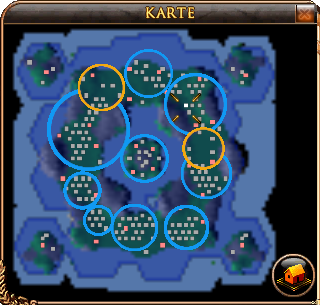
\includegraphics{decentralization_map_edited}
\vspace{1cm}

\subsection{First Contact}
\label{sec:firstcontact}

Depending on the map, mission and skill set of the participants, you will encounter your enemies earlier or later. In any case, you will want to have the better military strength. To boost your likelihood of winning fights  early in the game, it's important to have a solid gold industry running. This ideally consists of 2 \hyperref[sec:goldmine]{Gold Mines}, 2 \hyperref[sec:coalmine]{Coal Mines} and 2 \hyperref[sec:mint]{Mints}, unless you are facing many enemies at the same time. If you cannot find any gold, you'll want to go for strength in numbers by training a whole lot of \hyperref[sec:private]{Privates}. However, before attacking an enemy, you should \textbf{always} check the \hyperref[sec:statisticsmilitary]{Military Strength statistics}, as well as the \hyperref[sec:statisticscoins]{Coins Produced statistics}. Those will tell you whether or not you will stand a chance. Anyways, if you've got \hyperref[sec:general]{Generals} while your enemy has not produced any coins yet (or just started doing so), attack as long as you have the advantage. If you see any gold infrastructure like \hyperref[sec:goldmine]{Mines}, \hyperref[sec:mint]{Mints} or even just a \hyperref[sec:storehouse]{Storehouse}, that's what you should be going for in the first place.

\section{Military}
\label{sec:military}

\subsection{Soldier Industry}

To fight you need to recruit and upgrade your soldiers. For this, there are two main approaches. The first one is pretty simple and straightforward, while the second one is very powerful and prevents you from sending \hyperref[sec:privates]{Privates} (or other low-level soldiers) into fight.

\subsubsection{General Farm}
\label{sec:generalfarm}

\textit{If using the Vikings addon, see also \hyperref[sec:generalfarmbuff]{General Farm Buff}.}

\vspace{12pt}

To recruit a single \hyperref[sec:private]{Private}, \hyperref[sec:smithy]{one Sword, one Shield} and one \hyperref[sec:brewery]{Beer} need to be in a single \hyperref[sec:storehouse]{Storehouse}, a private will spawn automatically. To level up Soldiers, all you need is a \hyperref[sec:mint]{Coin} in a military building. One Soldier of every level gets promoted by one (i.e. if you have one of each \hyperref[sec:private]{Private}, \hyperref[sec:corporal]{Corporal}, \hyperref[sec:sergeant]{Sergeant} and \hyperref[sec:officer]{Officer}, all of them get promoted.

Of course, you could just let the coins be delivered directly to the front. However, it's much more efficient if you only allow coins in one building near the Headquarter, so you can let \hyperref[sec:private]{Privates} come in and let them promote, then throw them out again. For this to work, you need to prefer weak defensive Soldiers in your global economy settings.

\subsubsection{General Generator}
\label{sec:generalgenerator}

As you might have noticed, the previous system has some drawbacks. Mainly you need to modify the global economy settings badly so that there will be only \hyperref[sec:private]{Privates} in your military buildings, unless you manage to train everyone to the maximum level. To avoid this, you can build a setup where everything required to recruit and promote a Soldier gets brought into a single \hyperref[sec:storehouse]{Storehouse}. For promotion, you should build a \hyperref[sec:watchtower]{Watchtower} or, preferably, a \hyperref[sec:stronghold]{Stronghold} connected to the \hyperref[sec:storehouse]{Storehouse}. To prevent \hyperref[sec:private]{Privates} from coming out, There shouldn't be a road to the rest of your civilization, so to transport goods but not people, you have to use a water road. Now, go to your \hyperref[sec:storehouse]{Storehouse} and block any Soldiers but \hyperref[sec:private]{Privates} from going in.
\vspace{12pt}
In the end, if you've got \hyperref[sec:brewery]{Beer}, \hyperref[sec:smithy]{Swords and Shields} in that exact \hyperref[sec:storehouse]{Storehouse}, a \hyperref[sec:private]{Private} will spawn, go to the connected \hyperref[sec:watchtower]{Watchtower} or \hyperref[sec:stronghold]{Stronghold} and upgrade to \hyperref[sec:general]{General} level. As one Soldier (if you want to prefer strong soldiers in your global economy settings, even though it shouldn't be needed when using this technique, you must wait until all soldiers got promoted. However, this is very inefficient as one Soldier of every level could get promoted otherwise) in the building becomes a \hyperref[sec:general]{General}, you can evacuate him so there's space for another \hyperref[sec:private]{Private}. The evacuated \hyperref[sec:general]{General} can't go back to the \hyperref[sec:storehouse]{Storehouse}, so he will search for the nearest road and go to a different \hyperref[sec:storehouse]{Storehouse}, \hyperref[sec:harbor]{Harbor}, or your Headquarter.

\vspace{0.5cm}
\includegraphics[width=\textwidth]{generalgenerator_crop}
\vspace{0.5cm}

This method should forbid non-\hyperref[sec:general]{Generals} from fighting at all while making Soldier promotion very quick.

\subsection{The Power of Scattershots}
\label{sec:powerofscattershots}

\hyperref[sec:scattershot]{Scattershots} often seem useless, as they rarely hit something, shoot really slow and are already out of range or destroyed when the building process finishes. Lastly, they eat up lots of stone. However, they can still be an important tool during battle.

First of all, check if you have enough stone. On some maps, stone is really spare, so building a scattershot can be fatal. If there is enough stone, however, there are situations where scattershots are really useful. Look at the following scenarios:

\begin{itemize}
    \item You have a frozen border with so much military on each side, that nobody can go through
    \item You have a worse military strength and are afraid of an enemy attack
    \item You need to buy time and could use scattershots in combination with \hyperref[sec:buildingcanceling]{building canceling}
    \item You want to settle an island, but it's occupied (only works if the enemy's military buildings are near the mainland and in range of the scattershot)
    \item You have the greater forces but want to save your \hyperref[sec:general]{Generals}
\end{itemize}

In each of these scenarios, you can use scattershots to either force action on the enemy side, kill hostile soldiers without actually attacking, or make the enemy afraid of coming closer due to the risk of getting shot at. When considering that - assuming you have dozens of stones lying around - the ammunition does not cost anything valuable, scattershots are a slow, but efficient way to win a battle.

To learn how exactly you should put them to use, read the technical section about \hyperref[sec:scattershot]{scattershots}.

\subsection{Military Tricks}
\label{sec:militarytricks}

The following section is a collection of useful tricks regarding military fights. Not only can you use them to your advantage, but you should also learn how to deal with them when applied by your opponents. Most of the concepts have crucial drawbacks that you must be aware of.

\subsubsection{Using weakened enemies as rampart}
\label{sec:militaryrampart}

When fighting against multiple enemies, situations can come up, where you just defeated a tribe and immediately get to face the next one. This can be very dangerous, as you are defending on new territory without much industry, while your enemy could be on familiar grounds. Additionally, you likely lost a bunch of soldiers in previous fights. Preventing this situation should be your top priority.

A possible technique is to leave a small corridor of the almost destroyed enemy along your realm's boundary. This way, the new enemy would have to attack through the weakened enemy to reach you. Note that this is most effective if the two enemy folks are on the same team.

\vspace{0.6cm}
\includegraphics[width=\textwidth]{militaryrampart_crop}
\textit{Yellow is being used by blue as rampart before hitting green}
\vspace{1cm}

If they're not in the same team though, you can still implement this technique by making the corridor a bit wider. Still, you have to get your \hyperref[sec:decentralization]{decentralized industry} up as fast as possible before your future opponent takes the remaining territory.

\subsubsection{Destroying Buildings}
\label{sec:destroyingbuildings}

In this game, you are \textbf{never} guaranteed to have greater military force than your opponents. That's why it's essential to have good backup strategies in case of you being overwhelmed. One such strategy is destroying military buildings before the enemy can take them.

Whenever you see one of your military buildings attacked with not many chances of survival, you need to check the cause of your loss. Examples would be a poorly distributed military (e.g. strong soldiers aren't where they're needed the most; buildings far from enemy territory are occupied, and so on). This needs to be resolved quickly, however, retaking the building should be doable. However, in situations when your general \hyperref[sec:statisticsmilitary]{military strength} is far worse than your enemy's, the newly captured building won't be retakeable and will make it easy to reach further into your domain, without you having any chance to recover, almost certainly sealing your doom.

\label{wastingenemyresourcesbydestroyingbuildings}
If you manage to destroy your buildings before losing the fight, you cause the enemy to waste costly time, as they need to create new buildings, likely at least a \hyperref[sec:watchtower]{Watchtower}, which takes quite long to build while also consuming valuable resources. To make even more out of this situation, read about \hyperref[sec:buildingcanceling]{canceling buildings}.

However, destroying military buildings is not always the best choice. Even if you have far less soldiers, there is a chance that you have some \hyperref[sec:general]{Generals} while your opponent only got \hyperref[sec:private]{Privates}. In this situation it may be smarter to let your troops fight to death, as they will kill far more Privates than your enemy can spare. Retaking the building can wait until some fresh soldiers are upgraded.

\subsubsection{Building Canceling}
\label{sec:buildingcanceling}

In the case of an enemy is arming next to your border, either because you just met for the first time, or the \hyperref[wastingenemyresourcesbydestroyingbuildings]{scenario} described in the \hyperref[sec:destroyingbuildings]{Destroying Buildings} section took place and you don't feel ready for contact, you can delay attacks as long as your shared border is quite narrow.

To pull this off, let your opponent build a military building next to your border. This is gonna be a \hyperref[sec:watchtower]{Watchtower} or \hyperref[sec:stronghold]{Stronghold}, most of the time. Those building take a long time to build, so you should have enough time to build a \hyperref[sec:barrack]{Barrack} on your side of the border, which should clearly be finished first. This will destroy your opponent's construction side, letting time and materials go to waste. To guarrantee being done first, even if the enemy's building is just a \hyperref[sec:guardhouse]{Guard House}, you can get a local \hyperref[sec:woodindustry]{wood industry} up, together with a \hyperref[sec:storehouse]{storehouse} containing soldiers.

After canceling the building you should destroy the barrack again to give your enemy room for another building. Especially bots won't learn out of this trick.

\subsubsection{Complete Erasure}
\label{sec:completeerasure}

No, this is no suicide advice. In some situations there just isn't another option than forcing your opponent to approach you slowly by creating new buildings. To accomplish this, you can first silently evacuate important goods from storehouses near the front and then destroy all military buildings in a medium to big distance to the border at once. This way you can try to recover your industry (see the \hyperref[sec:minesandfoot]{Mines and Food} and \hyperref[sec:decentralization]{Decentralization} sections) and possibly overwhelm your enemy due to hurried \hyperref[sec:overexpansion]{overexpanding}.

Note, however, that this can greatly damage your economy if important mines are destroyed in the process. Make sure you got alternatives running \textbf{before} erasing.

\section{Food Systems}
\label{sec:foodsystems}

There are mainly 4 types of food:

\begin{itemize}
  \item Fish
  \item Bread
  \item Ham (\hyperref[sec:hunter]{Hunter})
  \item Ham (\hyperref[sec:slaughterhouse]{Slaughter})
\end{itemize}

\subsection{Fish}
\label{sec:fish}

Fishing is a great way to get food in the early game. One \hyperref[sec:fisherman]{Fisherman} produces \textbf{roughly} one fish every 190 seconds. Therefore you need 4 \hyperref[sec:fisherman]{Fisherman} to keep a single mine running. Depending on your \hyperref[sec:startresources]{starting resources}, you will have a total of 3, 6 or 12 fishers available right at the beginning. Make sure you don't exceed this limit, as investing metal to employ more fisherman is just not worth it when compared to other food systems.

Note, that fishing is non-renewable.

\subsection{Bread}
\label{sec:bread}

Bread is the best source of food during the game. It's renewable and you only need one \hyperref[sec:bakery]{Bakery} to keep a \hyperref[sec:mine]{Mine} running, as both buildings take 49 seconds to produce a good. To keep a \hyperref[sec:bakery]{Bakery} running you need one \hyperref[sec:mill]{Mill}, to keep that running you need about 1.75 \hyperref[sec:farm]{Farms}. The \hyperref[sec:bakery]{Bakery} also demands one bucket of water. Luckily, the \hyperref[sec:well]{Well Worker} also takes exactly 49 seconds to work. That being said, a great ratio for a bread system is 7 \hyperref[sec:farm]{Farms}, 4 \hyperref[sec:mill]{Mills}, 4 \hyperref[sec:bakery]{Bakeries} and 4 \hyperref[sec:well]{Wells}.

This system can feed 4 \hyperref[sec:mine]{Mines} for just 11 tools in total.

\subsection{Ham (Hunter)}
\label{sec:hamhunter}

The  \hyperref[sec:hunter]{Hunter} can roughly produce one ham every 70 seconds under optimal conditions. While that is about thrice as fast as the fisherman, you usually don't get more than 20 ham for a big area, as animals don't renew at all. Hunters can be great for gaining some food very early in the game, however, they're not worth considering anymore as you invest in other food systems.

\subsection{Ham (Slaughter)}
\label{sec:hamslaughter}

The second option to produce ham also works along with \hyperref[sec:farm]{Farms}, just like the \hyperref[sec:bread]{Bread System}. The \hyperref[sec:pigfarm]{Pig Farmer} grows one pig every 62 seconds, just like the \hyperref[sec:slaughterhouse]{Slaughter} kills a pig every 62 seconds. A \hyperref[sec:pigfarm]{Pig Farmer} needs wheat and water to feed his pigs, giving those right to the \hyperref[sec:slaughterhouse]{Slaughter}. Therefore the optimal ratio consists of 9 \hyperref[sec:farm]{Farms}, 7 \hyperref[sec:pigfarm]{Pig Farms}, 5 \hyperref[sec:well]{Wells} and 7 \hyperref[sec:slaughterhouse]{Slaughterhouses} to feed about 5,5 mines.

This renewable system uses up 16 tools in total.

\subsection{Food System Comparison}
\label{sec:foodsystemcomparison}

As the \hyperref[sec:fish]{Fish based system} (takes 4 tools per mine, non-renewable) and the \hyperref[sec:hamhunter]{Ham producing, Hunter-based system} (very short living, non-renewable) aren't well suited for a rich ore economy, this comparison mainly focuses on the renewable \hyperref[sec:bread]{Bread based-} and \hyperref[sec:hamslaughter]{Meat-producing, Slaughter-based system}.

Here is a direct comparison of the optimal ratios of both systems in terms of \textbf{tool efficiency}, \textbf{production efficiency}, \textbf{amount of buildings} and \textbf{amount of spots} taken (This means, a Tier 1 building takes 1 spot, a Tier 2 building takes 2 spots and a Tier 3 building takes 3 spots. This is not an in-game mechanic, but rather a way to summarize the Tier efficiency of a system), calculated down to feed a single mine of any type:

\begin{itemize}
  \item Bread requires 2,75 tools per mine while Ham takes up $2.\overline{90}$
  \item Bread feeds exactly 4 mines with a setup while Ham can feed about 5.5, adding unnecessary complexity
  \item Bread takes 4,75 buildings per mine while Ham requires $5.\overline{09}$
  \item Bread takes 10,25 spots per mine while Ham requires $12.\overline{18}$
\end{itemize}

As you can see, the \hyperref[sec:bread]{Bread system} wins every time and should therefore always be chosen over the \hyperref[sec:hamslaughter]{Meat-based alternative}.

\section{Ships and Harbor}
\label{sec:shipsandharbor}

\subsection{The Harbor}
\label{sec:harbor}

\textit{See also: \hyperref[sec:harbor_building]{Harbor (Building)}}\\

The \hyperref[sec:building_harbor]{Harbor} is the first step to discovering \hyperref[sec:islands]{Islands} in The Settlers II - 10th Anniversary. It acts just like every ordinary \hyperref[sec:stockhouse]{Stockhouse}, just that it has the ability to transfer goods and workers over to \hyperref[sec:ships]{Ships}. To send a Ship to discover a new \hyperref[sec:islands]{Island}, you must prepare a mission in the harbor's UI. This will get 4 \hyperref[sec:plank]{Planks}, 6 \hyperref[sec:stone]{Stones} and 1 \hyperref[sec:constructor]{Constructor} reserved into the harbor. If a {Ship} is ready, these things will get loaded onto the ship and you can select a direction where the ship should look for a place in the \hyperref[sec:ships]{ship's UI}.

\subsection{Ships}
\label{sec:ships}

\textit{See also: \hyperref[sec:shipyard]{Shipyard}}\\

Ships are made in the \hyperref[sec:shipyard]{Shipyard}. When ready for a mission, which was started previously in the \hyperref[sec:harbor]{Harbor} UI, you can select a direction where the ship should look for a Harbor when clicking on it. You can also cancel the Mission if there are no available Harbors.

\subsection{Goods Transport}
\label{sec:goodstransport}

When a building demands something, the nearest \hyperref[sec:stockhouse]{Stockhouse} is asked to bring the goods over. If there is no Stockhouse with the required good reachable over land and the demanded good is just coming out of a factory, this will go to the demanding building. Otherwise, the game will check for the item on an \hyperref[sec:islands]{Island}. If there is one, the item will be brought to the Islands \hyperref[sec:harbor]{Harbor} and will then eventually be brought to the Island or Mainland requesting the item via a \hyperref[sec:ships]{Ship}. To ensure a flowing good exchange, there should be at least 2 or 3 Ships dedicated to each Island.

The same concept also applies to settlers. However, those can randomly get stuck on islands. See \textit{\hyperref[sec:buildersstuckonisland]{Bug: Builders stuck on an island}}.

\section{Tips and Tricks}
\label{sec:tipsandtricks}

Finally, we come to the Tips and Tricks section. Here you'll find helpful concepts that will make your life a little (or a lot) easier. For each trick, you will find a score of the impact this trick can have in a game. You should decide how much you are willing to do to optimize your gameplay.

\subsection{Marking Mining Spots}

\textit{Impact rating: 6/10 (efficiency boost especially on large maps)}\\

When a geologist discovers a new ore that you do not immediately need, you can mark the ore as such by placing a \hyperref[sec:mines]{mine} building without connecting it to your road system. Whenever you do need that ore, go to the \hyperref[sec:economybuildings]{buildings economy settings tab} (press "B" on the keyboard) and click on the desired mine.\\

On the other hand, when one of your mines is exhausted, you can destroy the mine but leave the flag. This way you know that this spot is already exhausted and don't need to send another geologist later in the game.

\subsection{Ghost Buildings}
\label{sec:ghostbuildings}

\textit{Impact rating: 1/10 (high effort, little impact, even on small maps with gold in the middle)}\\

Ghost buildings are a technique that allows you to build mainly small buildings at the beginning of a new game at a higher speed by ensuring resources to be delivered a little quicker. Mainly useful for barracks as initial expansion can be accelerated.
To pull this off, first block the resources you want to be delivered quickly from the headquarter. Second, place any building that requires the resources you want to be delivered quickly (e.g. a \hyperref[sec:lookouttower]{lookout tower}) near the buildings that should receive them. This is the ghost building. Whenever the resources for the ghost building are almost there, destroy the final road to the ghost building. Now the resources are lying around some flags near the ghost building and cannot go back to the headquarter. Now you can place the buildings you want to be built accelerated, and the required materials will be delivered a little quicker as they are already lying around near the target.

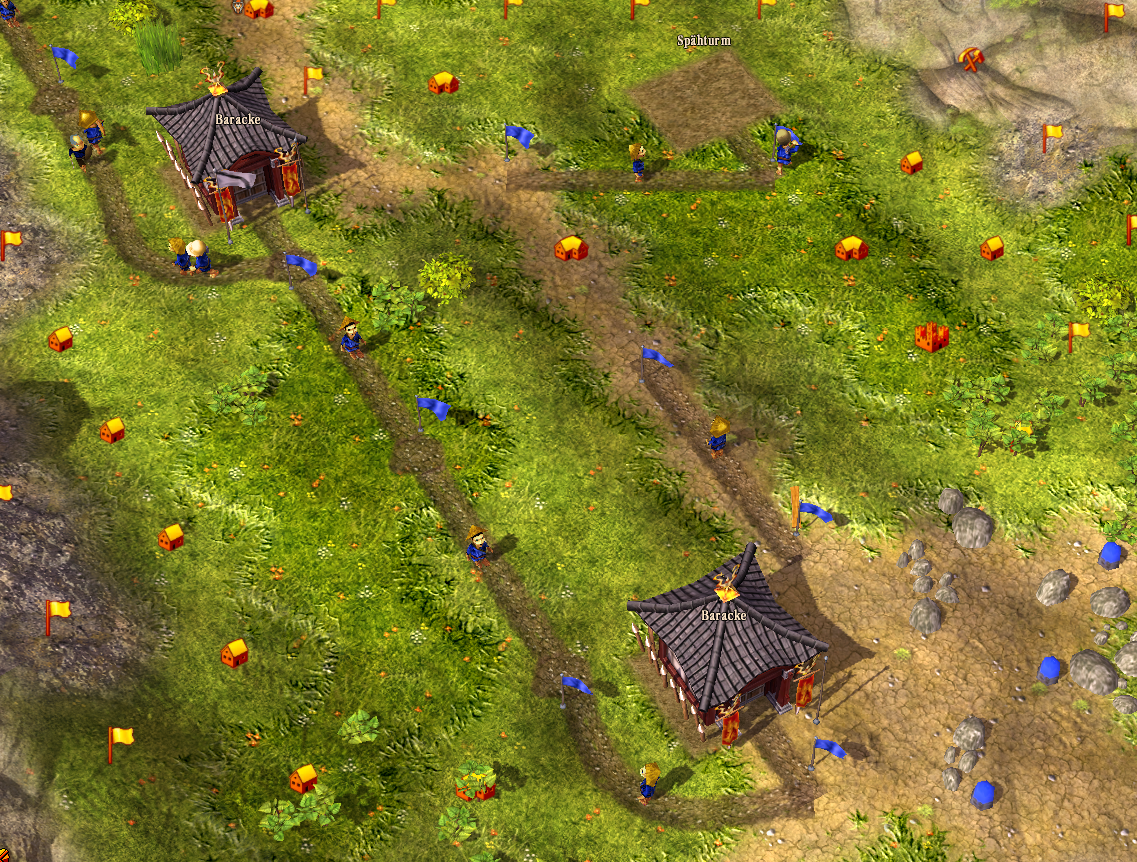
\includegraphics[width=\textwidth]{ghostbuilding_crop}

\textit{A barrack is being built using materials from a ghost lookout tower.}


\section{Common Pitfalls}
\label{sec:commonpitfalls}

When there is so much strategy involved, there's also lots of room for errors. Here you will learn about common pitfalls you need to avoid, some being more fatal than others.

\subsection{Beginner Struggles}
\label{sec:beginnerstruggles}

The following describes common issues and solutions I learned while being new to the game, as well as when introducing new players.

These will be ordered from early to later during a game.

\subsubsection{Wood Issues}
\label{sec:woodissues}

This is something even more experienced players can struggle with sometimes. At the beginning of a game, one of the most important resources is wood. You need it for every single building in the game, as well as for \hyperref[sec:ships]{Ships} and \hyperref[sec:metalworks]{Tools}. Especially at low \hyperref[sec:startingresources]{starting resources}, wood is spare when starting a new game. While you can get infinite wood from a good \hyperref[sec:woodindustry]{wood industry}, it's not always easy to get one up. If not enough wood is produced at the beginning, or even no wood at all (e.g. when other building were prioritized so there's no wood left for \hyperref[sec:woodcutter]{woodcutters} and \hyperref[sec:sawmill]{sawmills}), nothing can be built anymore and you're stuck during the part of the game where time matters the most. To solve this issue, other buildings need to be destroyed so the remaining can be used to build up wood producers.

As this is something you definitely must avoid, you have to make sure to follow the \hyperref[sec:woodindustry]{wood industry section} before spending the valuable resource elsewhere.

\subsection{Intermediate Issues}
\label{sec:intermediateissues}

Now follows a collection of things intermediate to advanced players should look after to optimize their gameplay. Note that these tips are not necessarily needed to win a game against bots. However, they will greatly enhance stability of everything you do.

\subsubsection{Over-Expansion}
\label{sec:overexpansion}

Over-Expansion often happens when one party claims a lot of enemy territory in a short time by taking military buildings and connecting them only with simple roads. There won't be many buildings aside from military, making the \hyperref[sec:minimap]{minimap} look empty. However, this visual issue is not the main problem with this approach.

Especially on big maps, over-expansion will cause the following problems.

\begin{itemize}
    \item Long transportation roads, making buildings take much longer to build or upgrade
    \item Replenishment soldiers taking long to arrive after a battle
    \item Carelessly created roads don't fit into a well-organized \hyperref[sec:roadsystem]{road system}
    \item Soldiers remain in buildings far from the front if those aren't emptied
    \item Makes leveling soldiers really hard when no \hyperref[sec:generalgenerator]{General Generator} is used
    \item Rapid expansion makes keeping track of natural resources (e.g. ore, fish) very hard
    \item Attacking too fast gets low-health \hyperref[sec:general]{generals} killed before they can heal
\end{itemize}

And possibly more.

The most dangerous points are the long transport ways. Without a \hyperref[sec:decentralization]{decentralized} economy near the borders you have a big disadvantage against an opponent with a more compact boundary, or a better distributed industry, possibly overwhelming you and forcing you into a \hyperref[sec:completeerasure]{complete erasure}.

To avoid this risk, make sure you don't attack too rapidly (unless strategically appropriate, e.g. when destroying gold industry or \hyperref[sec:storehouse]{storehouses}) and instead care about each chunk of new territory as much as you would when discovering new land by \hyperref[sec:expanding]{expanding} regularly.

\subsubsection{Forgetting to turn off the Metalworks}
\label{sec:forgettingmetalworks}

Usually, you won't need the \hyperref[sec:metalworks]{metalworks} working all the time, as the iron could be invested into \hyperref[sec:soldiers]{Soldiers} instead. Therefore, turning it on whenever needed (e.g. when building new \hyperref[sec:farm]{farms}) is a completely valid approach. However, one should not forget to turn it off again after the required tools are produced. While this can waste medium amounts of iron, it also delays soldier production, depending on the \hyperref[sec:waredistribution]{ware distribution economy setting}. It's safest to wait in front of the metalworks until enough tools are produced.

\subsubsection{No Stone}
\label{sec:nostone}

Certain maps don't have a lot of stone available, sometimes even just one stone field per party. Especially with low starting resources, this usually causes problems mid-game when building a \hyperref[sec:foodsystems]{food system} that requires a large amount of stone, or when creating many \hyperref[sec:harbor]{harbors}. The only two ways to get more stone when your natural resources are exhausted are trying to destroy enemy \hyperref[sec:stonemine]{stone mines} and mining the remaining yourself, and destroying buildings that required stone to be built. Good examples of these are enemy military buildings that you occupied. In the late game, destroying unneeded farms can also do the trick.

While it is generally possible to get more stone this way, it requires you to be stronger than your opponents. Since this can't be ensured all the time, you should instead try to be as spare on stone as possible. This includes the following:

\begin{itemize}
    \item Don't use scattershots
    \item Don't accidentally build the wrong building
    \item Don't build stone-heavy buildings when you don't actually need them (e.g. the \hyperref[sec:fortress]{fortress})
    \item Always let the materials be recovered when destroying buildings (i.e. don't destroy the flag)
    \item Don't keep stone in endangered \hyperref[sec:storehouse]{storehouses}
    \item Don't build more \hyperref[sec:harbor]{harbors} than needed
\end{itemize}

Be aware that these things do not harm - and are sometimes even great ideas - when enough stone is available.

Additionally, you can make profit out of your enemy's stone issues. Whenever you got the upper hand, you should target the storehouses containing stone (e.g. next to a stone mine) and they will be unable to enhance their \hyperref[sec:soldiers]{soldier industry}.

\subsection{Bugs}
\label{sec:bugs}

As The Settler II (10th anniversary) never really got any content updates, there are some minor, but gameplay-impacting bugs you should be aware of.

\subsubsection{Builders stuck on an Island}
\label{sec:buildersstuckonisland}

When using \hyperref[sec:shipsandharbor]{ships and the harbor} to bring your forces to an island, you will want to build up a decentralized industry at some point. Unfortunately, there's a little bug that could make \textbf{all} your builders and/or \hyperref[sec:leveler]{levelers} stuck on an island when requesting a new building, and no one on the island is ready to take the job. While normally, workers would go back to the mainland when needed there, in this case, they don't. This will completely freeze progress on your mainland and other islands. To fix this, build a \hyperref[sec:storehouse]{storehouse} and send the workers to it, out of the harbor. After all are in the storehouse, allow them to go back to the harbor and they will go back to the mainland when needed.

Note that while this mostly happens to builders and levelers, all workers that can be demanded by an island could be affected by this, including soldiers.

To generally prevent this from happening it's advisable to request a \hyperref[sec:storehouse]{Storehouse} right when building a harbor. While this doesn't seem to entirely prevent this bug from happening, it allows you to quickly send the workers to the storehouse to free them.

\section{Bonus}
\label{sec:bonus}

\subsection{Bonus A: Challenges}
\label{sec:challenges}

\subsubsection{In a Rush}
\label{sec:challenge_rush}

This one isn't too hard, however, it allows you to practice your skills in quickly building up a solid economy using low starting resources and no stone piles available.

\begin{itemize}
    \item Map: Fight2 (Odd map file name, it's the 8th entry in the dropdown menu, before "Paradise Island")
    \item \hyperref[sec:startingresources]{Starting Resources}: Low
    \item Win Condition: Defeat all Enemies
    \item Fog of War: On
    \item Enemies: All in the same team, highest difficulty
\end{itemize}

Your goal should be to be by far the first at the large gold deposits in the center and immediately start mining with a food economy already set up. This is also the perfect map to use \hyperref[sec:ghostbuildings]{Ghost Buildings}. Additionally you could try not to produce any soldiers but only using the 25 from your starting resources.

Challenges like this can really unveil wether you understood the \hyperref[sec:gettingstarted]{Getting Started} section and are able to apply it properly.

\subsubsection{The Ultimate Challenge}
\label{sec:challenge_ultimate}

You really studied the game and want to show off your skills using an incredibly hard challenge? This one's for you.

\begin{itemize}
  \item Map: Paradise Island
  \item \hyperref[sec:startingresources]{Starting Resources}: Medium
  \item Win Condition: Defeat all Enemies
  \item Fog of War: On
  \item Enemies: All in the same team, highest difficulty
\end{itemize}

This challenge is really hard because you need to defeat 5 Enemies all by yourself. Because this map is so huge (240*240 Spots) you cannot just rush your enemies. You need to play smart and for resources. Remember, they got five times as many as you did. Especially Iron will be tough, make sure you don't lose any of your soldiers before letting them become \hyperref[sec:general]{Generals}.

\subsubsection{The Ultimate Ultimate Challenge}
\label{sec:challenge_ultimate_ultimate}

You beat the last challenge? Good job! But there's more. This time you got even harder goals:

\begin{itemize}
  \item Map: Paradise Island
  \item \hyperref[sec:startingresources]{Starting Resources}: Low
  \item Win Condition: None (Endless Game)
  \item Fog of War: On
  \item Enemies: All in the same team, highest difficulty
  \item HQs: All randomized
  \item Custom Goal: Completely destroy every Enemy, make sure no one's got any territory left
\end{itemize}

As you can see, not only have your \hyperref[sec:startingresources]{Starting Resources} halved, the Headquarters are also randomized and, most importantly, you can't just chill on the main island erasing your opponents. You must dominate on every single island as well (there are 7 in total). However, as soon as you got your fleet ready to take the outer (and inner) land, you should never ever run out of resources again.

\subsubsection{More}
\label{sec:challenge_more}

Surely those challenges were hard. However, they're not impossible! You can always look for custom maps, or even make your own one! Playing with other experts can also be quite challenging. You found a really, really (and I mean really) hard or even impossible challenge? Why not share it by \hyperref[sec:contributing]{Contributing}.

\subsection{Bonus B: Vikings addon}
\label{sec:vikings}

The Vikings (german: Wikinger) addon for The Settlers II - 10th anniversary was released 2007 in the german language. While it mainly comes with a new race and a second campain path, it also brings some other minor changes, some of which can sustainably change gameplay.

The following is a non-exhaustive list of changes.

\begin{itemize}
  \item Added 3 New Bonus Maps
  \item Coin delivery is now turned off by default when building or claiming a new military building
  \item Added a "Soldaten hier ausbilden" (Train Soldiers here) button inside every \hyperref[sec:stockhouse]{Stockhouse}, \hyperref[sec:harbor]{Harbor} and the Headquarter. Weapons and beer will now exclusively be delivered to that building.
  \item An economy \hyperref[sec:messages]{Message} is sent, warning the player when Soldier count in storehouses drops below 20
  \item An economy Message is sent, warning the player when plank or stone count in storehouses drops below 20
  \item The \hyperref[sec:hunter]{Hunter} now emits a no resources found economy message
  \item New orange map indicators now signal certain events:
    \begin{itemize}
      \item Building constructed (circle)
      \item Military building manned (circle)
      \item Campain Quest target (cross)
      \item Attack or defense ended, no matter the outcome (fire)
      \item Building emits a no resources found economy message (circle)
    \end{itemize}
    Additionally, the position of ships is now permanently visible on the map through ship markers.
  \item Added new Viking \hyperref[sec:ships]{Ship} names
  \item An economy message is sent when there's a traffic jam around a flag
  \item An economy message is sent when a new tool was produced
  \item Buildings now drop remaining resources stored inside when destroyed
  \item Combat messages are now sent when an attack fails, and when a defense was successful
  \item Apparently, raw materials now prefer local industry buildings more reliably
     \begin{itemize}
       \item Potential bug: Soldier preference is ignore if a storehouse with different soldiers is closer to the building
     \end{itemize}
  \item [UI] The mouse wheel can now be used to change sliders
\end{itemize}

Most of those are clearly informational or cosmetic, but some can really make a difference in gameplay.

\subsubsection{General Farm buff}
\label{sec:generalfarmbuff}

Multiple changes make building a \hyperref[sec:generalfarm]{General Farm} arguable easier and more effective. Those include the new coin delivery default, the "Train Soldiers here" button and the potential soldier bug.

Due to the new coin delivery default, it's now much easier to ensure that only the dedicated building is capable of receiving coing. The new button removes the necessity of disallowing weapons, beer and coins in every storehouse except for the right one (which, of course, not only applies to the General Farm). However, most interesting is the new bug, which can be abused as feature.

To explain in detail, the bug causes the "Prefer strong/weak Soldiers" economy setting to only take a secondary effect. Whatever storehouse is the closesd to the military building sends its soldiers out - no matter if strong or weak. If there are both strong and weak soldiers in the storehouse, the economy setting decides. While this is really annoying when generals are further away from the demanding building than privates, as it's nearly impossible to allocate the right soldiers without evacuating storehouses, it can be really useful in the situation of a General Farm.

If you know that you will only have one shared border where strong soldiers frequently have to go to - which definitely can't be assured on many maps, in that cases it's best to continue using the farm as without the Vikings addon - you can build two \hyperref[sec:storehouse]{Storehouses} around your Watchtower or Fortress that is used to promote soldiers. One must be in the direction of the enemy border and the other in the opposite direction. Make sure the first one is \textbf{further} away from the military building than the second. Now, dedicate the second storehouse to train soldiers using weapons and beer. It should also hold the coins needed to promote soldiers. Additionally \textbf{disallow} generals to be in that storehouse. The storehouse near the enemy border should disallow all soldiers but generals. The economy soldier preference should still prefer weak soldiers to allow kicking soldiers out of the military building more efficiently.

\vspace{0.4cm}
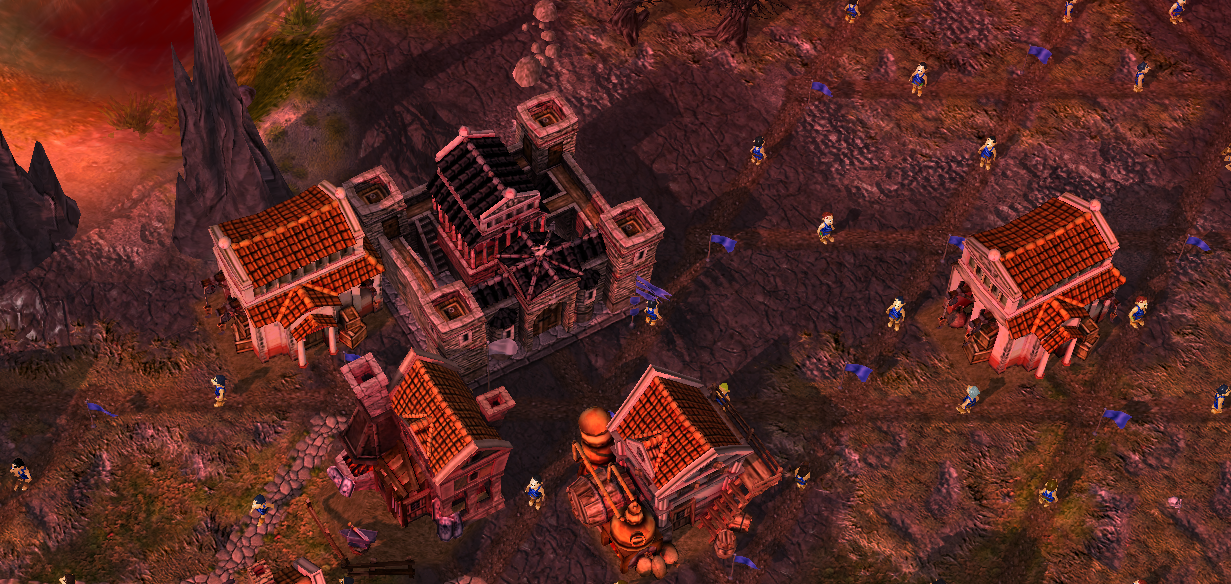
\includegraphics[width=\textwidth]{improved_general_farm}
\vspace{0.1cm}

This setup results in the following process:

\begin{itemize}
  \item Privates are recruited in the inner storehouse
  \item Privates go into the military building
  \item They're promoted to Generals
  \item When kicked, they are forced to go into the further away storehouse
  \item That storehouse being further away ensures that only privates enter the military building
  \item Because they're closer to the border, Generals will be preferred when a military building near the border demands soldiers
\end{itemize}

The other General Farm limitations do apply. E.g., Privates can still be sent into fight when there are no Generals available. That's why it's still advisable to use a \hyperref[sec:generalgenerator]{General Generator} instead, which also benefits from the new recruitment storehouse button.

\end{document}
